\newpage
\chapter{Fluxo de Gradiente em Espaços de Wasserstein}

Neste capítulo mostraremos como EDPs podem ser expressadas como
fluxos de gradiente em um espaço de Wasserstein
(i.e. espaço métrico de medidas de probabilidades com distância
de Wasserstein)\footnote{A principal referência para este capítulo
é \citet{santambrogio2017euclidean}.}. A exposição é
focada em apresentar de maneira clara e sucinta o necessário para entendimento
do assunto, sem provar os resultados mais refinados, o que tornaria o
texto muito extenso e de difícil
entendimento\footnote{Fluxo de gradientes é uma área por si só, assim, sugerimos ao leitor nesta área
que consulte \citet{ambrosio2008gradient}}. Assim, restringimos
nossa exposição ao caso de $\mathbb R^n$. Note, porém, que muitas das definições
utilizadas podem ser facilmente estendidas para espaços de Hilbert.

Seja uma função $F:\mathbb R^n \to \mathbb R \in C^1$, e $x_0 \in \mathbb R^n$,
onde queremos descobrir $x(t)$ que resolve o seguinte sistema de equações:
\begin{equation}
    \begin{cases}
        x'(t) = -\nabla F(x(t)), \ t>0,\\
        x(0)  = x_0.
    \end{cases}
\end{equation}
A solução $x(t)$ do sistema acima será uma curva iniciando em $x_0$ e se movendo
na direção de menor gradiente, ou seja, a solução é dada
pelo famoso algoritmo de descida de gradiente. Em outras palavras,
a solução $x(t)$ caracteriza um fluxo de gradiente\footnote{Essa definição é informal. O conceito
de fluxo de gradiente será formalizado na seção seguinte.}.
Um exemplo desse tipo de solução é mostrado na Figura \ref{fig:fluxogradiente}

\begin{figure}[H]
\begin{center}
    \includegraphics[width=0.8\textwidth]{./Figures/fluxogradiente}
\end{center}
    \caption{Exemplo de fluxo de gradiente onde $F(x,y) = x^2 + 0.2 y^2$,
    com ponto inicial $(x(0),y(0)) = (1.0,1.0)$. A superfície representa os valores
    de $F(x,y)$, enquanto que as esferas vermelhas representam a solução do fluxo de gradiente
    com um \textit{time-step} de $0.1$. Perceba que a ``velocidade'' do fluxo é proporcional ao 
    gradiente, como pode ser visto pelo espaçamento decrescente entre cada uma das esferas.}
    \label{fig:fluxogradiente}
\end{figure}

Esse problema é simples quando estamos em espaços de dimensão finita e com
funções diferenciáveis, porém, torna-se mais
interessante e complexo quando começamos a considerar espaços de dimensão infinita
como $\mathcal P_2(\mathbb R^n)$. Neste cenário, temos que repensar, por exemplo,
a ideia de gradiente, já que não está mais claro que seria o gradiente quando
$x(t) = \rho_t \in \mathcal P_2(\mathbb R^n)$. Além disso, $F$ não é mais uma
função de $\mathbb R^n$ em $\mathbb R$, mas um funcional atuando em medidas
de probabilidade.

É interessante observar que, uma vez que consigamos reformular EDPs
como fluxos de gradiente em Wasserstein, poderemos utilizar resultados
obtidos nessa área para provar, por exemplo, existência e unicidade.

\section{Introdução ao Fluxo de Gradiente}

\subsection{Definições Iniciais}

Antes de formalizar a ideia de fluxo de gradiente, vamos introduzir alguns
conceitos de análise convexa que são necessárias para tratar
do assunto de maneira rigorosa.

\begin{definition}[Subdiferencial]
    Seja $f:\mathbb R^n \to (-\infty, +\infty]$ própria, ou seja, $f(x) \neq +\infty \forall x$.
    O subdiferencial de $f$ é dado por:
    \begin{equation}
        \partial f(x) := \{p \in \mathbb R^n:
        f(y) \geq f(x) + \langle p, y-x\rangle, \forall y \in \mathbb R^n
        \}.
    \end{equation}
    Se $p \in \partial f(x)$, então $p$ é um subgradiente de $f$ no ponto $x$.
\end{definition}
A intuição por trás da definição
de subdiferencial é ilustrada na Figura \ref{fig:subdiferencial}.
Note que se a função $f$ for convexa e diferenciável, teremos que $\partial f(x) = \{\nabla f(x)\}$.
Porém, caso a função não seja convexa, não haverá essa garantia. Assim, é comum usar essa ideia de
subdiferencial somente em funções convexas.

Uma primeira generalização dessa ideia de subdiferencial pode ser usada em funções que chamamos
de semi-convexas, ou $\lambda$-convexas. Muitos resultados de fluxo de gradientes podem ser
aplicados a essa classe maior de funções, que, como apontado por \citet{santambrogio2017euclidean},
cobrem vários casos de interesse (e.g. em conjuntos limitados,
todas as funções $f \in C^2$ serão semi-convexas).

\begin{definition}[$\lambda$-Convexidade]
    Uma função $f:\mathbb R^n \to (-\infty,+\infty]$ é $\lambda$-convexa
    para um $\lambda\in\mathbb R$ se
    \begin{equation}
        g(x):=f(x) -\frac{\lambda}{2}|x|^2
    \end{equation}
    for convexa.
    Note que se $f$ for $\lambda$-convexa com $\lambda =0$, temos que a função é convexa.
    Se $\lambda <0$, a noção é mais fraca que convexidade e implica que
    $f$ tem sua parte negativa com crescimento no máximo quadrático.
    Finalmente, se $\lambda > 0$, a função é estritamente convexa e
    limitada inferiormente.
\end{definition}

\begin{definition}[$\lambda$-Subdiferencial]
    Seja $f:\mathbb R^n \to (-\infty, +\infty]$ própria, e $\lambda \in \mathbb R$.
    O $\lambda$-subdiferencial de $f$ é dado por
    \begin{equation}
        \nabla_\lambda f(x) := \{
            p \in \mathbb R^n: f(y) \geq f(x) + \langle p, y-x\rangle
            + \frac{\lambda}{2}|y-x|^2, \forall y \in \mathbb R^n\}.
    \end{equation}
\end{definition}

Podemos generalizar ainda mais essa noção de subdiferencial com a seguinte definição.
\begin{definition}[Subdiferencial Generalizado]
    \footnote{\citet{ambrosio2021lectures} chama de Gateaux subdifferencial.}
    Seja $f:\mathbb R^n \to (-\infty, +\infty]$ própria, ou seja, $f(x) \neq +\infty \forall x$.
    O subdiferencial generalizado de $f$ é dado por:
    \begin{equation}
        \partial_G g(x):= \{p \in \mathbb R^n: \liminf_{t\to 0^+}\frac{f(x+tv) - f(x)}{t}
        \geq \langle p,v \rangle v \in \mathbb R^n\}.
    \end{equation}
    Onde $t \to 0^+$ simboliza que $t$ tendo a $0$ pela direita.
    Note que $\nabla f(x)\subset \nabla_\lambda f(x) \subset \nabla_G f(x)$, com igualdade
    das três caso $f$ seja convexa.
\end{definition}

\begin{figure}[H]
    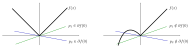
\includegraphics[width=1\textwidth]{./Figures/subdiferencial}
    \caption{Exemplo de subdiferencial. Perceba que considerando
    o subdiferencial generalizado, teríamos
    $p_1 \in \partial_G f(0)$ e $p_2 \in \partial_G f(0)$ para as duas imagens.}
    \label{fig:subdiferencial}
\end{figure}

Agora podemos definir de forma rigorosa o fluxo de gradiente.

\begin{definition}[Fluxo de Gradiente]
    Seja $f:\mathbb R^n \to \mathbb R$.
    Assim, dizemos que $x:(0,+\infty) \to \text{Dom}(f)$ é um fluxo de gradiente
    de $f$ se $x \in \text{AC}_{\text{loc}}((0,+\infty), \mathbb R^n)$ e
    \begin{equation}
        x'(t) \in - \nabla_G f(x(t)), \quad \text{para } \lambda\text{-a.e } t \in (0,+\infty),
    \end{equation}
    onde $\lambda$ é a medida de Lebesgue. Note que dizemos que $x$ começa em $x_0$ se
    $\lim_{t \to 0^+} x(t) = x_0$.
\end{definition}

\subsection{Resultados Básicos de Existência e Unicidade}

Uma vez introduzida a ideia de fluxo de gradiente, vamos agora provar alguns
resultados básicos relacionados ao sistema de equações

\begin{equation}
    \begin{cases}
        x'(t) \in -\partial F(x(t)), \ \text{para quase todo } t>0,\\
        x(0)  = x_0.
    \end{cases}
    \label{eq:fluxograd}
\end{equation}

Veja que agora a função $F$ não é mais necessariamente derivável. Este cenário
é bem menos restrito que o que apresentamos logo no início do capítulo.

\begin{lemma}
    Seja $f:\mathbb R^n \to \mathbb R \cup \{+\infty\}$ convexa, $p_1 \in \partial f(x_1)$
    e $p_2 \partial f(x_2)$. Então
    \begin{equation}
        \langle p_1 - p_2, x_1 - x_2 \rangle \geq 0.
    \end{equation}
\end{lemma}
\begin{prf}
    Pela definição de subdiferencial, temos que
    \begin{align*}
        &p_1 \in \partial f(x_1) \implies f(x_2) \geq f(x_1) + \langle p_1, x_2 - x_1\rangle\\
        &p_2 \in \partial f(x_2) \implies
        f(x_1) \geq f(x_2) + \langle p_2, x_1 - x_2\rangle.
    \end{align*}
    Assim, somando as duas equações, temos que
    \begin{align*}
        &f(x_2) + f(x_1) \geq f(x_1) + f(x_2) +
        \langle p_1, x_2 - x_1\rangle
        \langle p_2, x_1 - x_2\rangle
    \end{align*}
    Rearranjando, obtemos
    \begin{align*}
        &0 \geq
        \langle p_1,x_2 \rangle
        -\langle p_2,x_1 \rangle
        \langle p_2,x_1 \rangle
        -\langle p_2,x_2 \rangle \\
        &\implies
        \langle p_1 - p_2 , x_1 - x_2 \rangle \geq 0.
    \end{align*}
\end{prf}

\begin{theorem}
    Seja $F:\mathbb R^n \to \mathbb R$ \textbf{convexa}, $x_0 \in \mathbb R^n$, e
    $x_1$ e $x_2$ duas soluções de \eqref{eq:fluxograd}.
    Então,
    \begin{equation}
        |x_1(t) - x_2(t)| \leq |x_1(0) - x_2(0)|, \ \forall t >0.
    \end{equation}
    Logo, a solução do sistema de equações é única.
\end{theorem}
\begin{prf}
    Primeiro, faça $g(t) = \frac{(x_1(t) - x_2(t))^2}{2}$, e toma a derivada em $t$. Assim
    \begin{equation*}
        g'(t) = \langle x_1(t) - x_2(t), x_1'(t) - x_2'(t) \rangle.
    \end{equation*}
    Usando o fato que
    $x_1'(t) \in \partial F(x_1(t))$ e
    $x_2'(t) \in \partial F(x_2(t))$, temos pelo lemma que acabamos de demonstrar que
    \begin{equation*}
        g'(t) = \langle x_1'(t) - x_2'(t) , x_1(t) - x_2(t) \rangle \geq 0.
    \end{equation*}
    Além disso, como ambas as soluções começam em $x_0$, temos que $g(0) = 0 \geq g(t)$, já que
    a derivada de $g(t)$ é sempre menor ou igual a zero. Portanto
    \begin{align*}
        g(t) = \frac{(x_1(t) - x_2(t))^2}{2} \leq 0 &\implies
        |x_1(t) - x_2(t)| \leq |x_1(0) - x_2(0)| = 0 
        \\
        &\implies
        x_1(t) = x_2(t).
    \end{align*}
\end{prf}

Podemos estender o resultado do teorema acima para o caso mais geral onde
$F$ é $\lambda$-convexa. A demonstração é bastante parecida, porém, um pouco mais convoluta.
Por conta disso optamos por apresentar os dois resultados de forma separada.

\begin{theorem}
    Seja  $F:\mathbb R^n \to \mathbb R$ \textbf{$\lambda$-convexa}, $x_0 \in \mathbb R^n$.
    Então o sistema de equações \eqref{eq:fluxograd} tem uma solução única.
    Além disso, se $\lambda >0$, a taxa de convergência para o mínimo global
    de $F$ é exponencial, ou seja, para $x^* = \argmin_{x\in \mathbb R^n} F(x)$
    \begin{equation}
        |x(t) - x^*| \leq e^{-\lambda t}|x(0)- x^*|,
    \end{equation}
    onde $x(t)$ é a solução.
\end{theorem}